\chapter{Darwinian Character Creation}

\begin{wrapfigure}{O}{\figwidth}
	\begin{center}
		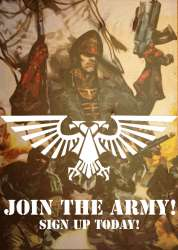
\includegraphics[width=\figwidth]{pics/1/1.jpg}
	\end{center}
\end{wrapfigure}

Our DM can be a little evil.

Last weekend our group got together for a marathon session to start a new campaign in a new system.
Upon arrival we were all given copies of the Only War sourcebooks and told to build a regiment, then build grunt level characters, then make a few backup characters.
Now our DM runs what we refer to as "High Mortality Games"(in our several year long DnD game so many PCs died that our GM actually appears on the "Hitler Scale" of death measurement) and we were all familiar with the nature of a guardsman's life, so each of us made a bunch of backups and didn't get too attached to any of our characters as we wrote them.
No special snowflakes here.

Our regiment was mustered, our characters met and trained, and we were deployed to fight some Orks. %TYPO orks -> Orks
We learned the system in a few skirmishes and commiserated when some of our characters rolled poorly or screwed up and bit the dust.
Then we were marched out to the trenches, given our piece of the line, and the battle started.


\begin{wrapfigure}{O}{\figwidth}
	\begin{center}
		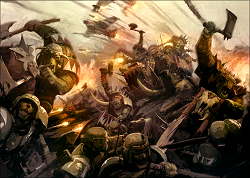
\includegraphics[width=\figwidth]{pics/1/2.png}
	\end{center}
\end{wrapfigure}
We had expected some sort of priority mission.
We had expected to be the heroes who went in behind the enemy, or were dispatched to save a key position, or led the valiant charge.
Instead we were put in a bloody trench and told to Hold The Line.

The Orks came and we killed them. 

The Orks came again and we killed them.

The Orks came again and we killed them, but now we were low on ammo.

The Orks came again and some of us died.

The Orks came again and brought a tank and the rest of us died, except for me, I ran.

The first session ended there, with our first set of characters dead in the trenches.
We agreed it was a proper introduction to the life of a 40k guardsman, and got ready for the next day's session where we expected to finally be sent on our mission.

\begin{wrapfigure}{O}{\figwidth}
	\begin{center}
		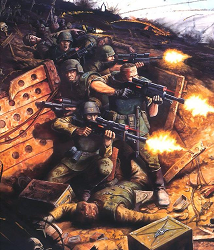
\includegraphics[width=\figwidth]{pics/1/3.png}
	\end{center}
\end{wrapfigure}
The second session started with us watching my character's execution by the Commissar.
Then we were put back in the same bloody trench and told to Hold The Line.
We did better this time, we actually held out long enough for fresh ammo and reinforcements to come up, but in the end we died.
Then we brought up new characters and did it again in another part of the trenches.
Then again.
Then again.

We were rolling up new characters between turns now, either to bring in as reinforcements or for when we had to start up as a new unit.
Very rarely we would survive long enough to be rotated to the rear or take a non-fatal injury and get evaced, usually we all died.
Finally after three in game days and dozens of character deaths we were told to Charge.

\begin{wrapfigure}{O}{\figwidth}
	\begin{center}
		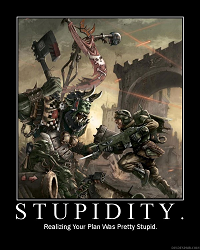
\includegraphics[width=\figwidth]{pics/1/4.png}
	\end{center}
\end{wrapfigure}
We bitched hard when we heard this, it was a death sentence.
Our characters had done well this time, we were all still alive and ammo levels were good.
We knew our squad could have held out much longer in our nice safe trenches.
Our DM asked us if we wanted to lodge our complaints In Character, so we shut up and Charged. 

We died like animals.

We fought on the left flank of the charge, then on the right, then got to play our first armored characters in the center.
When the charge failed we played as a basilisk crew covering the retreat. Then our regiment was rotated off the front.

Our regiment had lost a third of its strength in that first engagement.
Out of dozens of characters only ten had survived, and five of those were artillerymen who never saw the enemy.
We were shown the battle map, we were shown where our squads held or failed, we were shown how our charge weakened the enemy for the fresh (and much more valuable) reserve troops to come up and break them.
We were given a summary of the next few months of light skirmishes and mustering, then we were sent into battle against Traitor Guard.

\begin{wrapfigure}{O}{\figwidth}
	\begin{center}
		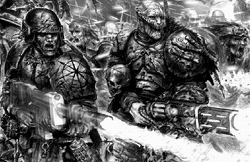
\includegraphics[width=\figwidth]{pics/1/5.png}
	\end{center}
\end{wrapfigure}
We were taking a city this time and once again our regiment acted as the cannon fodder.
We secured and pushed, and secured and pushed, and died and died and died.
We decided we'd take the Orks back any day, at least with them it was obvious who the enemy was and their snipers and heavy weapons teams were NOTHING compared to what we were fighting here.
We were higher level this time and better at the game, but still we died in droves leaving only a few characters alive when our regiment was stood down while a veteran regiment took the lead.

Once again we got to see the nice little map of our progress, and we all got a warm fuzzy feeling when he showed us how our stubborn defense of one building had crippled an enemy advance, but we were exhausted.
Our DM pressed us to play fast and make new characters faster. 
We would roll up Lil Jimmy who lied about his age to enlist, then have him bleeding out in a pile of rubble within a handful of minutes. 
It drained us. 
We were actually glad to take the evening off from playing to just watch movies and hang out.

\begin{wrapfigure}{O}{0.5\textwidth}
	\begin{center}
		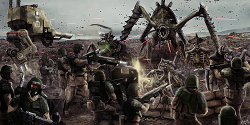
\includegraphics[width=0.5\textwidth]{pics/1/6.png}
	\end{center}
\end{wrapfigure}
The final day of our marathon started with more Orks, but this time we won. That's not to say we didn't die like frogs in a blender, but we damn well won. We pushed them out of their barricades and hounded them across the plains when they routed. I played a gunner in a salamander during the chase and mowed down greenskins like ugly blades of grass. We partied like champs in the tiny redneck town we liberated, then settled in for a few months of boring garrison duty before we got redeployed. Then we fought some Tyranids.

It was only a splinter fleet so we actually had a chance, but it was hell. 
Our regiment was defending an evac point on some grassy agri-world and it was trench work again. 
We burned off the grass to clear lines of fire, dug ourselves into the rich soil, set up the heavy weapons, and watched the edge of the burn area like hawks.
 Trigger-happy hawks as it turned out, we wound up failing a spot-check and killing the first few retreating PDF to come through the grass. 

When the Tyranids came it was ridiculous. 
We mowed down wave after wave of Gaunts, but unlike Orks Tyranids don't lose morale and break, they just keep coming as fast as you can kill them. %TYPO gaunts -> Gaunts
We stopped using actual dice for a while, just so we could roll combat faster.

\begin{wrapfigure}{O}{\figwidth}
	\begin{center}
		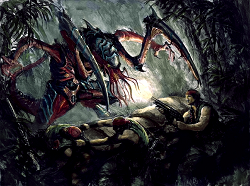
\includegraphics[width=\figwidth]{pics/1/7.png}
	\end{center}
\end{wrapfigure}
The bastards in command had decided to do a "Collapsing Defence", which meant we fought until the front trench was collapsing, then they shelled the bejeezus out of us while we retreated. 
We lost something like 20 PCs to our own gorram shells, but it really did work pretty well, at least until we ran out of ground to give. 
All the civvies were out, it was just a few regiments of guard crammed into a spaceport completely surrounded by the swarm.
We were killing them off as fast as possible and hoping that either reinforcements or evac would come down before ammo ran out.

Things started to get bad when the higher forms of Tyranid started appearing. 
Gaunts and gargoyles are bad enough, but it was when the warriors showed up that we started taking serious casualties. 
The evac shuttles had started to ferry men up and we had some actual air support, unfortunately our regiment was going to be the rear guard. 
The end was in sight and morale was holding up well, right up until we encountered a Lictor brood, then things started to fall apart. 

I hate Lictors, I bloody hate them. 
We played three backline squads in a row and each one was torn to bloody shreds by those sneaky bastards, all without us landing a kill. 
We started to rout, but our Commissar and his guards went into the breach, killed one of them, and shouted the regiment back into position.

\begin{wrapfigure}{O}{\figwidth}
	\begin{center}
		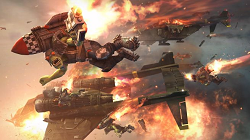
\includegraphics[width=\figwidth]{pics/1/8.png}
	\end{center}
\end{wrapfigure}
Our evac finally came and what was left of our regiment started the final retreat. 
There were a few valiant last stands, but most of us managed to get to the shuttles. 
Our final squad had just boarded and was taking off when the air interdiction broke down and Tyranid air units started attacking the shuttles.

We were equal parts pissed and terrified as our DM described shuttle after shuttle being destroyed. 
The Regimental Commander's bird was nailed early, so were the bigger shuttles with the vehicles. 
He didn't say who was in most of the other shuttles, just rolled his dice and removed them from the board as they fell. 
It was heartbreaking.

Finally there was only one shuttle left. 
Even though the Tyranid fliers swarmed it, none of their shots seemed to hit and it started to climb out of the atmosphere. 
Then it was away, the fliers broke off and that one shuttle was headed for its fleet transport, free and clear.

\begin{wrapfigure}{O}{\figwidth}
	\begin{center}
		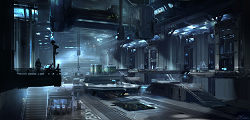
\includegraphics[width=\figwidth]{pics/1/9.png}
	\end{center}
\end{wrapfigure}
Inside the shuttle our last set of characters was trying to figure out what the hell was going on. 
There were about fifty guardsmen crammed into a twenty man shuttle and no one was telling us anything. 
We had all heard the Tyranid fliers attacking and everyone felt it when we hit space. 
The guardsmen close to the cockpit relayed what they could overhear from the pilot's radio, so everyone knew that the other shuttles had been attacked but no one was sure exactly what happened.
In any case we were all happy to be alive and were looking forward to getting off the crowded shuttle, then the shuttle stopped. 
The guardsmen near the cockpit told us we were being redirected to a different transport and the pilots did not look happy.

When the shuttle docked everyone piled out and we found ourselves in a completely empty loading bay. 
An order came via the speaker system to form up by rank for inspection, at this point our GM gave us a list of the guardsmen who were on the shuttle. 
Every single character who had survived a battle had been on the shuttle along with a few other grunts. 
All 37 of our beloved guardsmen had lived! (With the exception of the artillery crew we played, but screw those guys, teamkilling jerks)

\begin{wrapfigure}{O}{\figwidth}
	\begin{center}
		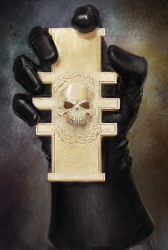
\includegraphics[width=\figwidth]{pics/1/10.png}
	\end{center}
\end{wrapfigure}
We formed up, and after a bit of waiting the doors opened then a few squads of storm troopers marched in and instructed us to drop our weapons.
There was a bit of argument on this point, until the captain of the stormtroopers pulled out an Inquisitorial Rosette and told us we were currently "guests" of the Ordos Xenos.

After we were done pissing ourselves and disarming, an acolyte and a team of medicae entered. 
We were informed that our regiment had been disbanded, we were officially dead, and we would all be subject to a scan for Genestealer infection. %TYPO: genestealer -> Genestealer

At this point our DM ended the session. 
We were each handed copies of the Dark Heresy core book, a list of our surviving guardsmen with all the filler grunts crossed off, and were told to pick our characters for the next game.

Yea, so that's how our DM does backstories.







